% Build twice here: pdflatex -interaction=nonstopmode -halt-on-error resume10An26w.tex
\documentclass[a4paper,10pt,pdflatex,ja=standard,jafont=ipaex-type1,
  magstyle=real,scale=1]{bxjsarticle}
\usepackage{lmodern}
\usepackage{amsmath,amssymb,mathtools}
\usepackage{geometry}
\geometry{reset,left=22mm,right=22mm,top=20mm,bottom=17mm,
  headheight=13pt,headsep=6mm,footskip=10mm}
\usepackage{xcolor}
\usepackage{enumitem}
\usepackage{array,booktabs,tabularx}
\usepackage{fancyhdr}
\usepackage{lastpage}
\usepackage{tikz}
\usetikzlibrary{arrows.meta,calc,decorations.pathreplacing}

\definecolor{ink}{HTML}{193A5C}
\definecolor{accent}{HTML}{237D82}
\definecolor{soft}{HTML}{EAF3F3}
\definecolor{muted}{HTML}{52616B}
\newcommand{\coursename}{解析学 II}
\newcommand{\handoutnumber}{10}
\pagestyle{fancy}
\fancyhf{}
\fancyhead[L]{\small\color{ink}\coursename{}・授業要約と演習}
\fancyhead[R]{\small\color{ink}第\handoutnumber 回}
\fancyfoot[C]{\small\color{ink}\thepage/\pageref{LastPage}}
\renewcommand{\headrulewidth}{0.3pt}
\setlength{\parindent}{0pt}
\setlength{\parskip}{2pt}
\setlength{\abovedisplayskip}{5pt}
\setlength{\belowdisplayskip}{5pt}
\setlength{\abovedisplayshortskip}{3pt}
\setlength{\belowdisplayshortskip}{4pt}
\setlist[itemize]{leftmargin=1.8em,itemsep=1pt,topsep=2pt,parsep=0pt}

\newcommand{\handouttitle}[1]{%
  \begin{center}
    {\Large\color{ink}#1}\par\vspace{3mm}
    {\color{accent}\rule{0.88\linewidth}{0.7pt}}
  \end{center}\vspace{-2mm}}
\newcommand{\handout}[2]{%
  \renewcommand{\handoutnumber}{#1}%
  \handouttitle{第#1回\quad #2}}
\newcommand{\topic}[1]{\par\vspace{5pt}%
  {\large\sffamily\mdseries\color{accent}#1}\par\vspace{2pt}}
\newcommand{\keybox}[1]{\par\vspace{3pt}\begingroup
  \setlength{\fboxsep}{4pt}%
  \colorbox{soft}{\parbox{\dimexpr\linewidth-2\fboxsep\relax}{\small #1}}%
  \endgroup\par\vspace{2pt}}
\newenvironment{problems}
  {\begin{enumerate}[leftmargin=2em,itemsep=3pt,topsep=3pt,parsep=0pt,
    font=\color{accent}]}
  {\end{enumerate}}


\newcommand{\examplelabel}[1]{{\sffamily\mdseries\color{ink}#1}}
\newcommand{\problemspace}{\par\vspace{5mm}}
\newcommand{\exercises}{%
  {\color{accent}\hrule height 0.7pt}\vspace{3pt}%
  \topic{演習問題（6題）}%
  {\small 領域と積分範囲を確認し、計算過程も書こう。図を描くと範囲を読み取りやすい。}\par}
\tikzset{
  handout diagram/.style={>={Stealth[length=3.2pt,width=3.2pt]},line join=round,
    every node/.style={font=\scriptsize,text=ink}},
  region/.style={fill=soft,draw=accent,semithick},
  slice/.style={accent,line width=1.8pt},
  guide/.style={muted,densely dashed,thin},
  axis/.style={->,ink,thin}}


% Review Q&A can also be used for actual student feedback when it is available.
\newcommand{\feedback}[2]{%
  \par\addvspace{8pt}\noindent\begin{minipage}{\linewidth}%
  {\color{ink}Q. #1}\par\vspace{2pt}%
  {\color{accent}A. }#2%
  \end{minipage}\par}

\begin{document}
\fontsize{10pt}{13.5pt}\selectfont
\setlength{\abovedisplayskip}{4pt}
\setlength{\belowdisplayskip}{4pt}
% Feedback section: add comments and responses here when available.
\fancyhead[L]{\small\color{ink}\coursename{}・フィードバック}
\handout{10}{前回のコメントへのフィードバック}
% \feedback{comment}{response}
\clearpage

% Previous small-test section: add the questions and solutions here.
\fancyhead[L]{\small\color{ink}\coursename{}・小テスト}
\fancyhead[R]{\small\color{ink}第9回}
\handouttitle{第9回\quad 小テスト}
% Questions and solutions are intentionally blank.
\clearpage

\fancyhead[L]{\small\color{ink}\coursename{}・授業要約と演習}
\fancyhead[R]{\small\color{ink}第\handoutnumber 回}
\handout{10}{スカラー場とベクトル場}\label{lesson-start}
\keybox{到達目標：勾配・発散・回転の入力と出力を区別し、場の局所的な変化を計算できる。
図の矢印と偏微分の式を対応させよう。}

\topic{場と微分演算子}
開集合 $U\subset\mathbb R^3$ 上の関数 $f:U\to\mathbb R$ をスカラー場、
$\vec F=(P,Q,R):U\to\mathbb R^3$ をベクトル場という。
以下、成分は $C^1$ 級とする。温度・密度はスカラー場、速度・力はベクトル場の例である。


\topic{勾配：スカラー場からベクトル場へ}
$$
 \nabla f=(f_x,f_y,f_z),\qquad
 D_{\vec u}f=\nabla f\cdot\vec u\quad(|\vec u|=1).
$$
方向微分の最大値は $|\nabla f|$。$\nabla f\ne0$ なら、最大になる方向は
$\vec u=\nabla f/|\nabla f|$ である。等位面 $f=c$ の正則点では $\nabla f$ は法線になる。
曲線 $\vec r(t)$ に沿う変化率は連鎖律により
$$
 \frac d{dt}f(\vec r(t))=\nabla f(\vec r(t))\cdot\vec r'(t).
$$


\par\vspace{2pt}\noindent
\begin{minipage}[b]{0.98\linewidth}\centering
\begin{tikzpicture}[handout diagram,x=0.65cm,y=0.65cm]
\foreach \radius in {0.5,1,1.5}{\draw[accent!60] (0,0) circle (\radius);}
 \draw[axis] (-1.8,0) -- (2.3,0) node[right] {$x$};
 \draw[axis] (0,-1.7) -- (0,1.9) node[above] {$y$};
 \fill[ink] (1,0) circle (1.6pt);
 \draw[->,ink,semithick] (1,0) -- (2,0) node[above] {$\nabla f$};
 \draw[->,accent,semithick] (1,0) -- (1,0.8) node[above right] {接線};
 \node[right] at (2.8,0.7) {$f=x^2+y^2$};
 \node[right] at (2.8,-0.2) {勾配は等位線に垂直};
\end{tikzpicture}\par
{\small\color{muted}勾配の方向へ進むと、関数値は最も速く増える}\par
\end{minipage}
\par\vspace{2pt}

\topic{発散と回転}
発散はスカラー場、回転はベクトル場を与える。
$$
 \operatorname{div}\vec F=\nabla\cdot\vec F=P_x+Q_y+R_z,
$$
$$
 \operatorname{curl}\vec F=\nabla\times\vec F
 =(R_y-Q_z,\ P_z-R_x,\ Q_x-P_y).
$$
速度場の発散は局所的な湧き出し・吸い込み、回転は局所的な渦の向きと強さを表す。
\par\examplelabel{例：$\vec F=(-y,x,0)$。}
$$
 \operatorname{div}\vec F=0,\qquad
 \operatorname{curl}\vec F=(0,0,2).
$$
発散が0でも、回転が0とは限らない。


\par\vspace{2pt}\noindent
\begin{minipage}[b]{0.48\linewidth}\centering
\begin{tikzpicture}[handout diagram,x=0.85cm,y=0.65cm]
\draw[axis] (-1.8,0) -- (1.85,0) node[right] {$x$};
 \draw[axis] (0,-1.65) -- (0,1.85) node[above] {$y$};
 \foreach \x in {-1,0,1}{\foreach \y in {-1,0,1}{
  \ifdim\x pt=0pt\ifdim\y pt=0pt\else
   \draw[->,accent] (\x,\y) -- ({1.4*\x},{1.4*\y});\fi
  \else\draw[->,accent] (\x,\y) -- ({1.4*\x},{1.4*\y});\fi}}
 \node[below] at (0,-1.7) {$\vec F=(x,y,0)$};
\end{tikzpicture}\par
{\small\color{muted}湧き出し：$\operatorname{div}\vec F=2$}\par
\end{minipage}\hfill
\begin{minipage}[b]{0.48\linewidth}\centering
\begin{tikzpicture}[handout diagram,x=0.85cm,y=0.65cm]
\draw[axis] (-1.8,0) -- (1.85,0) node[right] {$x$};
 \draw[axis] (0,-1.65) -- (0,1.85) node[above] {$y$};
 \foreach \x in {-1,0,1}{\foreach \y in {-1,0,1}{
  \ifdim\x pt=0pt\ifdim\y pt=0pt\else
   \draw[->,accent] (\x,\y) -- ({\x-0.38*\y},{\y+0.38*\x});\fi
  \else\draw[->,accent] (\x,\y) -- ({\x-0.38*\y},{\y+0.38*\x});\fi}}
 \node[below] at (0,-1.7) {$\vec F=(-y,x,0)$};
\end{tikzpicture}\par
{\small\color{muted}回転：$\operatorname{curl}\vec F=(0,0,2)$}\par
\end{minipage}
\par\vspace{2pt}

\newpage
% Keep the remaining summary in the upper half of page 2.
\noindent\begin{minipage}[b][\dimexpr0.5\textheight-\parskip\relax][t]{\linewidth}
\topic{ポテンシャルと恒等式}
$\vec F=\nabla\phi$ と書けるとき、$\phi$ をスカラーポテンシャルという。
$C^2$ 級の $\phi$、$\vec A$ について、混合偏微分の交換から
$$
 \nabla\times(\nabla\phi)=\vec0,\qquad
 \nabla\cdot(\nabla\times\vec A)=0.
$$
$\vec F=\nabla\times\vec A$ と書けるとき、$\vec A$ はベクトルポテンシャルである。
星形の開集合上では、$C^1$ 級の $\vec F$ に対する $\operatorname{curl}\vec F=\vec0$ は
スカラーポテンシャルの存在を導く。領域に穴がある場合は、この条件だけでは十分でない。


星形とは、ある点 $a\in U$ から各点 $x\in U$ への線分が、すべて $U$ に含まれること。

\topic{例：ポテンシャルを成分から求める}
$\vec F=(2xy,x^2,0)$ に対して $\phi_x=2xy$ を積分すると
$\phi=x^2y+h(y,z)$。残りの成分から $h_y=h_z=0$ なので
$$
 \phi=x^2y+C,\qquad \nabla\phi=(2xy,x^2,0).
$$
\keybox{勾配・発散・回転の入力と出力を確認する。ポテンシャルの存在を判断するときは、場の微分だけでなく領域の条件も調べる。}

\par\vspace{2pt}\noindent
\begin{minipage}[b]{0.48\linewidth}\centering
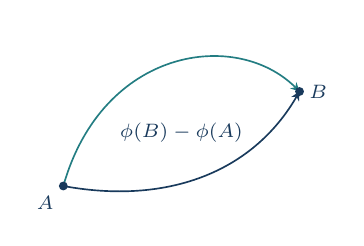
\begin{tikzpicture}[handout diagram,x=1cm,y=0.8cm]
\coordinate (A) at (0,0); \coordinate (B) at (3,1.5);
 \draw[->,accent,semithick] (A) .. controls (0.5,2.2) and (2.2,2.5) .. (B);
 \draw[->,ink,semithick] (A) .. controls (1.3,-0.3) and (2.4,0.2) .. (B);
 \fill[ink] (A) circle (1.6pt) node[below left] {$A$};
 \fill[ink] (B) circle (1.6pt) node[right] {$B$};
 \node at (1.5,0.85) {$\phi(B)-\phi(A)$};
\end{tikzpicture}\par
{\small\color{muted}勾配の場では、積分は端点だけで決まる}\par
\end{minipage}\hfill
\begin{minipage}[b]{0.48\linewidth}\centering
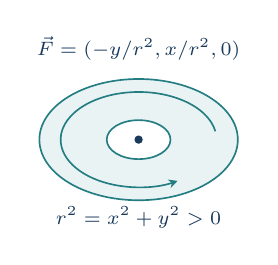
\begin{tikzpicture}[handout diagram,x=0.9cm,y=0.55cm]
\path[region,even odd rule] (0,0) circle (1.4) (0,0) circle (0.45);
 \draw[accent,->,semithick] (10:1.1) arc[start angle=10,end angle=300,radius=1.1];
 \fill[ink] (0,0) circle (1.5pt);
 \node at (0,-1.8) {$r^2=x^2+y^2>0$};
 \node[above] at (0,1.6) {$\vec F=(-y/r^2,x/r^2,0)$};
\end{tikzpicture}\par
{\small\color{muted}軸を除いた領域：回転は0でも循環は $2\pi$}\par
\end{minipage}
\par\vspace{2pt}

\end{minipage}\par\nointerlineskip
% Keep the exercises and writing space in the lower half of page 2.
\noindent\begin{minipage}[b][0.5\textheight][t]{\linewidth}
\exercises
\begin{problems}
\item $f=x^2+2y^2+3z^2$ の勾配を求めよ。点 $(1,1,1)$ における最大の方向微分と、その方向の単位ベクトルを求めよ。
\problemspace

\item $\vec F=(xy,yz,zx)$ の発散と回転を計算し、それぞれがスカラーかベクトルかを確認せよ。
\problemspace

\item $\vec F=(yz,xz,xy)$ の発散・回転を求め、スカラーポテンシャルを一つ求めよ。
\problemspace

\item $f=x^2-y^2+z^2$ の $\nabla f=\vec0$ となる点を求めよ。その点が極大・極小か、座標軸上での関数値を比較して判断せよ。
\problemspace

\item $C^2$ 級の $f$ に対して $\nabla\times(\nabla f)=\vec0$ を、成分ごとに混合偏微分を用いて示せ。
\problemspace

\item $\vec F=(-y,x,0)$ のベクトルポテンシャルを、$\vec A=(0,0,h(x,y))$ の形で一つ求めよ。また、この $\vec F$ がスカラーポテンシャルをもたない理由を述べよ。
\problemspace
\end{problems}
\end{minipage}

\newpage
\handouttitle{第10回\quad 演習問題の解答}
{\small 設定した範囲と条件も確認しながら、計算を振り返ろう。}\par
\begin{problems}
\setlength{\itemsep}{7pt}
\item $\nabla f=(2x,4y,6z)$。点 $(1,1,1)$ では $(2,4,6)$ となり、
最大の方向微分は $\sqrt{4+16+36}=2\sqrt{14}$。
その方向の単位ベクトルは $(1,2,3)/\sqrt{14}$ である。

\item 成分ごとに微分すると
$$
 \operatorname{div}\vec F=y+z+x,\qquad
 \operatorname{curl}\vec F=(-y,-z,-x).
$$
発散は実数を値とするスカラー場、回転は3成分のベクトル場である。

\item $\operatorname{div}\vec F=0$、$\operatorname{curl}\vec F=\vec0$。
ポテンシャルは $\phi=xyz$ と取れる。実際、
$$
 \nabla(xyz)=(yz,xz,xy)=\vec F.
$$
この場は $\mathbb R^3$ 全体で定義されている。

\item $\nabla f=(2x,-2y,2z)=\vec0$ となるのは原点だけ。
しかし $f(t,0,0)=t^2>0$、$f(0,t,0)=-t^2<0$（$t\ne0$）なので、
原点のどの近傍にも正の値と負の値がある。原点は極大でも極小でもなく、鞍点である。

\item $f\in C^2$ では混合偏微分が交換できるため、各成分は
$$
 \nabla\times(\nabla f)
 =(\partial_y\partial_zf-\partial_z\partial_yf,\
   \partial_z\partial_xf-\partial_x\partial_zf,\
   \partial_x\partial_yf-\partial_y\partial_xf)=\vec0.
$$
これで3成分すべてが0であることが確かめられた。

\item $\vec A=(0,0,h)$ に対して $\nabla\times\vec A=(h_y,-h_x,0)$。
$h=-(x^2+y^2)/2$ とすれば
$$
 \vec A=\left(0,0,-\frac{x^2+y^2}{2}\right),\qquad
 \nabla\times\vec A=(-y,x,0)=\vec F.
$$
一方、$\nabla\times\vec F=(0,0,2)\ne\vec0$ なので、
この $\vec F$ を勾配として表すスカラーポテンシャルは存在しない。
\end{problems}
\keybox{発散0と回転0は別々の条件。回転0からポテンシャルの存在を結論するときは、定義域に関する仮定も必要になる。}
\end{document}
